\documentclass[tikz,border=8pt]{standalone}
\usepackage{tikz}
\usetikzlibrary{arrows.meta,positioning,fit}

\tikzset{
  layer/.style={
    draw,
    rounded corners=2pt,
    thick,
    align=center,
    minimum width=3.3cm,
    minimum height=1.2cm,
    font=\small,
    fill=orange!10
  },
  head/.style={
    layer,
    fill=green!10
  },
  io/.style={
    layer,
    fill=gray!12
  },
  flow/.style={
    -{Latex[length=2.6mm]},
    thick
  }
}

\begin{document}
\begin{tikzpicture}[node distance=0.95cm]
  \node[io] (input) {Input mel\\$1 \times M \times T$};
  \node[layer, right=of input] (stem) {Stem\\Conv $1 \rightarrow 16$, $3 \times 3$, stride $1$\\BatchNorm + ReLU};
  \node[layer, right=of stem] (b1) {Residual Block 1\\main: $16 \rightarrow 16 \rightarrow 16$\\skip: identity\\output $16 \times M \times T$};
  \node[layer, right=of b1] (b2) {Residual Block 2\\main: $16 \rightarrow 32 \rightarrow 32$\\first conv stride $2$\\skip: $1 \times 1$, stride $2$\\output $32 \times \frac{M}{2} \times \frac{T}{2}$};
  \node[layer, right=of b2] (b3) {Residual Block 3\\main: $32 \rightarrow 64 \rightarrow 64$\\first conv stride $2$\\skip: $1 \times 1$, stride $2$\\output $64 \times \frac{M}{4} \times \frac{T}{4}$};
  \node[head, right=of b3] (avg) {AdaptiveAvgPool2d\\output $1 \times 1$\\$64 \times 1 \times 1$};
  \node[head, right=of avg] (flat) {Flatten\\$64$};
  \node[head, right=of flat] (fc1) {Linear\\$64 \rightarrow 64$};
  \node[head, right=of fc1] (relu) {ReLU};
  \node[head, right=of relu] (drop) {Dropout\\$p=0.2$};
  \node[head, right=of drop] (fc2) {Linear\\$64 \rightarrow \mathrm{out\_dim}$};

  \draw[flow] (input) -- (stem);
  \draw[flow] (stem) -- (b1);
  \draw[flow] (b1) -- (b2);
  \draw[flow] (b2) -- (b3);
  \draw[flow] (b3) -- (avg);
  \draw[flow] (avg) -- (flat);
  \draw[flow] (flat) -- (fc1);
  \draw[flow] (fc1) -- (relu);
  \draw[flow] (relu) -- (drop);
  \draw[flow] (drop) -- (fc2);

  \node[draw, dashed, rounded corners=3pt, inner sep=6pt, fit=(stem)(b3), label=above:{\small Residual Feature Extractor}] {};
  \node[draw, dashed, rounded corners=3pt, inner sep=6pt, fit=(avg)(fc2), label=above:{\small Classification Head}] {};
\end{tikzpicture}
\end{document}
